\newpage
\chapter{Transformation Zeitreihe zu Netzwerk}
Ziel unseres Forschungsprojektes war es verschiedene Algorithmen zur dynamischen Ausreißer Erkennung in Netzwerken, auf Zeitreihen anzuwenden. Um dies zu ermöglichen müssen die Zeitreihen hierzu zunächst in Netzwerke umgewandelt werden. In diesem Kapitel wird dieser Schritt erläutert. Je nach Algorithmus der verwendet werden soll, wird die Umwandlung unterschiedlich durchgeführt. Aus diesem Grund ist dieses Kapitel in weitere Unterkapitel aufgegliedert um auf die Besonderheiten bei der Umwandlung für unterschiedliche Algorithmen einzugehen.
\section{Netsimile}
\label{chap:trsnsNeti}
Der Netsimile Algorithmus erwartet für jeden Zeitabschnitt ein Netzwerk. Sodass später die einzelnen Netzwerke miteinander verglichen werden können um auffällige Netzwerke zu identifizieren. Hierzu muss die Zeitreihe zunächst in unterschiedliche Zeitabschnitte aufgeteilt werden. Je nach Datensatz kann hierbei ein unterschiedliches Intervall zum aufsplitten der Zeitreihe gewählt werden. Insofern die Zeitreihe eine Periodizität aufweist, kann diese bestimmt und als Intervall festgelegt werden.\\ 
Anschließend muss jeder Zeitabschnitt in ein Netzwerk umgewandelt werden. Dies wird getan indem die Ähnlichkeit zwischen allen Elementen des Zeitabschnitts berechnet wird. Die Ähnlichkeiten bilden anschließend die Gewichte zwischen den Elementen im Netzwerk.
$$D_{ij}=\left(\sum_{k} \left|v_{k}^{i}-v_{k}^{j}\right|^{p}\right)^{1/p}$$
Das Ergebnis hiervon bildet eine Adjazenzmatrix. Diese Adjazensmatrix muss anschließend in ein Textfile geschrieben werden, sodass die Daten vom Netismile Algorithmus genutzt werden können. Dazu wird für jede Kante eine neue Zeile im File generiert, in dieser wird zunächst der Ursprungsknoten, dann der Zielknoten und anschließend die Gewichtung aufgeführt. Für jeden Zeitabschnitt muss ein einzelner File angelegt werden. 

\begin{figure}[H]
	\centering
	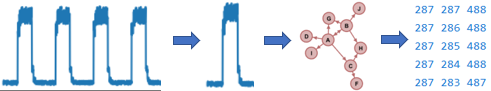
\includegraphics[width=13cm]{fig/tsToNet/tsToCsv}
	\caption{Umwandlung einer Zeitreihe in Netzwerk}
	\label{img:tsToNet}
\end{figure}
\workTodo{Das Netzwerk aus der Grafik noch abändern}



\section{MIDAS}
\label{chap:trsnsMidas}
Die Umwandlung in eine Zeitreihe funktioniert ähnlich wie in \autoref{chap:trsnsNeti}. Lediglich das Übergabeformat an den Algorithmus unterscheidet sich. Hierbei muss nicht für jeden Zeitabschnitt eine neue Datei angelegt werden. Anstatt dessen muss bei jeder Kante angegeben werden in welchem Abschnitt sie stattfindet. Außerdem kann an den Algorithmus nicht direkt eine Gewichtung der Kante übergeben werden. Es muss anstatt eine Gewichtung zu übergeben einfach 10 mal die gleiche Kante übergeben werden. Je nachdem wie hoch die Gewichtung der Kante ist.

\begin{figure}[H]
	\centering
	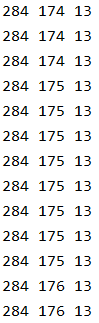
\includegraphics[width=2cm]{fig/tsToNet/midasData}
	\caption{Datensatz Midas}
	\label{img:tsToNetMiData}
\end{figure}
\workTodo{Vielleicht kleineren Auszug aus Datensatz verwenden}


\section{MIDAS-R}
\label{chap:trsnsMidasR}
\workTodo{Hab hier das mit der Hauptkomponentenzerlegung gemacht. Wenn es Ergebnisse hierfür gibt. Kann ich das hier noch erklären}
